\section{Analyse von Funktion F226: Ausleihfrist abgelaufen}
Falls die Leihdauer eines Dokumentes abgelaufen ist, wird der Mailtext aus der 
Datenbank abgerufen und an die E-Mail Adressen der beiden Entleiher(Bürge/Entleiher) gesendet.

Hierfür muss eine neue App erstellt werden, welche alle benötigten Informationen enthält bzw. sich aus der Datenbank holt, um diese Funktion zu bewerkstelligen.
Diese Funktion gehört zur Komponente \textbf{Models}, natürlich in Interaktion mit \textbf{DB}.
\begin{figure}
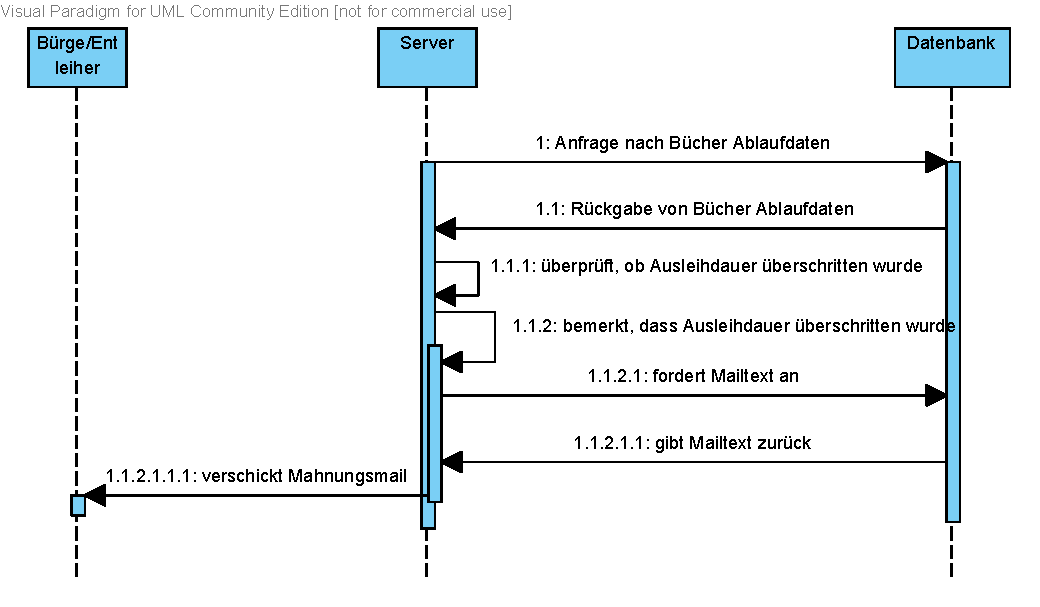
\includegraphics[width=0.8\linewidth]{bilder/SeqMail.pdf}
\caption{Sequenzdiagramm: Ausleihfrist abgelaufen}
\label{fig:226}
\end{figure}

\section{Analyse von Funktion F227: Ausleihhistory}
\label{f:227}
Die Ausleihhistory ist eine Liste von Personen, welche bereits ein bestimmtes Dokument ausgeliehen hatten bzw.\ immer noch haben.
Es wird ein Filter über die Dokument-Objekte gelegt, damit nur bestimmte bzw.\ das gewünschte Dokument und deren bisherige Ausleiher ausgegeben werden. Diese so erhaltenen Daten müssen nun noch durch ein Frontend-View an geeigneter Stelle der Web-Seite angezeigt werden.
Diese Funktion ist eine Built-In-Funktion von Django und wird über \textbf{View} benutzt. Da die Informationen widerrum nur in der Datenbank liegen, muss diese Komponente bei jeder Anfrage auf \textbf{DB} zugreifen.
Das Sequenz-Diagramm wird hier nicht dargestellt, da es eine einfache Suchanfrage an die DB mit anschließendem, gefilterten Ergebnis ist, siehe auch Abb.\ \ref{fig:Seqü}.

\section{Analyse von Funktion F228: Derzeitiger Leihender}
\label{f:228}
Die Funktion Derzeitiger Leihender gibt die Person aus, welche gerade ein bestimmtes Buch ausgeliehen hat.
Da in Django die User durch eine eigene Klasse dargestellt werden, muss diese Klasse auf die Rechte des momentan angemeldeten Benutzers überprüft werden. Falls diese Rechte ausreichend sind, wird wiederum durch ein Queryset+Filter die jeweiligen Dokumente und der dazugehörige Leihende durch einen View ausgegeben.
Auch diese Funktion benutzt die Komponente \textbf{View} in Zusammenhang mit \textbf{DB} (siehe auch \ref{f:227} \nameref{f:227}).
Auch hier wird auf eine Angabe des Sequenzdiagrammes verzichtet, da es wie auch in \ref{f:227} \nameref{f:227} eine einfache gefilterte Suchanfrage ist.



\section{Analyse von Funktion F229: Entleihliste}
Wenn der Benutzer angemeldet ist, ist er im Stande, sich alle seine momentan entliehene Dokumente als Liste anzeigen zu lassen.

Diese Funktion greift auf die Komponente \textbf{View} zu, um die Informationen dafür zu erhalten, muss vorher jedoch auf die \textbf{DB} zugegriffen werden.
Das Sequenzdiagramm für diese Funkton wird hier nicht angegeben, siehe \ref{f:227} \nameref{f:227} oder \ref{f:228} \nameref{f:228}.
